\chapter{Sprint 2 : Traitement et consultation des données}
\newpage
\section{Introduction}

Le quatrième chapitre présente les fonctionnalités développées dans le Sprint 2. Nous y décrivons la gestion des factures, la consultation des résultats d’extraction, les tableaux de bord ainsi que la configuration des seuils de l’intelligence artificielle.

\section{Backlog du Sprint}

\renewcommand{\arraystretch}{1.25}

\begin{table}[H]
	\centering
	\footnotesize
	
	\begin{tabularx}{\textwidth}{|c|p{3.6cm}|c|X|c|}
		\hline
		
		\rowcolor{blue!20}
		\textbf{ID} &
		\textbf{User Story} &
		\textbf{ID-US} &
		\textbf{Tâche} &
		\textbf{Estimation}
		\\ \hline
		
		%====================================================
		
		\multirow{4}{*}{2.1}
		& \multirow{4}{3.6cm}{
			En tant que comptable, je veux consulter les résultats d’extraction afin de vérifier les données extraites.
		}
		& 2.1.1 & Conception UML de consultation des extractions. & \multirow{4}{*}{2 jours}
		\\ \cline{3-4}
		
		& & 2.1.2 & Développement de l’interface de consultation.
		& \\ \cline{3-4}
		
		& & 2.1.3 & Implémentation backend d’affichage des résultats.
		& \\ \cline{3-4}
		
		& & 2.1.4 & Tests et validation.
		& \\ \hline
		
		%====================================================
		
		\multirow{4}{*}{2.2}
		& \multirow{4}{3.6cm}{
			En tant que comptable, je veux gérer les factures selon leurs statuts afin de suivre leur traitement.
		}
		& 2.2.1 & Conception UML de gestion des factures. & \multirow{4}{*}{2 jours}
		\\ \cline{3-4}
		
		& & 2.2.2 & Développement de l’interface des statuts.
		& \\ \cline{3-4}
		
		& & 2.2.3 & Implémentation backend de gestion des statuts.
		& \\ \cline{3-4}
		
		& & 2.2.4 & Tests et validation.
		& \\ \hline
		
		%====================================================
		
		\multirow{4}{*}{2.3}
		& \multirow{4}{3.6cm}{
			En tant que comptable, je veux consulter le tableau de bord afin de visualiser les indicateurs et statistiques.
		}
		& 2.3.1 & Conception du tableau de bord. & \multirow{4}{*}{2 jours}
		\\ \cline{3-4}
		
		& & 2.3.2 & Développement des graphiques et indicateurs.
		& \\ \cline{3-4}
		
		& & 2.3.3 & Intégration des statistiques dynamiques.
		& \\ \cline{3-4}
		
		& & 2.3.4 & Tests et validation.
		& \\ \hline
		
		%====================================================
		
		\multirow{4}{*}{2.4}
		& \multirow{4}{3.6cm}{
			En tant qu’administrateur, je veux définir les seuils de confiance de l’IA afin d’adapter le traitement automatique.
		}
		& 2.4.1 & Conception UML de configuration IA. & \multirow{4}{*}{1 jour}
		\\ \cline{3-4}
		
		& & 2.4.2 & Développement de l’interface de configuration.
		& \\ \cline{3-4}
		
		& & 2.4.3 & Implémentation backend des seuils IA.
		& \\ \cline{3-4}
		
		& & 2.4.4 & Tests et validation.
		& \\ \hline
		
	\end{tabularx}
	
	\caption{Backlog détaillé du Sprint 2}
	\label{tab:backlog_sprint2}
	
\end{table}

\FloatBarrier


%====================================================
\section{Analyse}

\subsection{Analyse fonctionnelle}

\subsubsection{Diagramme de cas d’utilisation}

Le diagramme de cas d’utilisation montre les fonctions principales du deuxième sprint. Le comptable consulte les résultats de l’extraction, le comptable gère les factures et le comptable utilise le tableau de bord. L’administrateur configure les seuils de confiance de l’IA.

\begin{figure}[H]
	\centering
	
\includegraphics[width=0.9\textwidth]{usecase_sprint2.jpg}
	\caption{Diagramme de cas d’utilisation du Sprint 2}
	\label{fig:usecase_sprint2}
\end{figure}

\FloatBarrier

%====================================================
\subsubsection{Description textuelle des cas d’utilisation}

\subsubsection*{Cas d’utilisation : Consulter les extractions}

\begin{table}[H]
	\centering
	\renewcommand{\arraystretch}{1.35}
	\rowcolors{2}{gray!10}{white}
	
	\begin{tabularx}{\textwidth}{|p{3.8cm}|X|}
		\hline
		\rowcolor{blue!20}
		\textbf{Use Case} & \textbf{Consulter les extractions} \\ \hline
		
		\textbf{Acteur} & Comptable \\ \hline
		
		\textbf{Description} & Le comptable peut consulter les résultats d’extraction automatique des factures. Les résultats affichent les données extraites, le statut et le score de confiance de l’IA. \\ \hline
		
		\textbf{Pré-condition} & Le comptable est authentifié et des factures ont été traitées par le système. \\ \hline
		
		\rowcolor{blue!10}
		\textbf{Scénario nominal} &
		1- Le comptable ouvre l’interface des extractions. \newline
		2- Le système récupère les résultats d’extraction disponibles. \newline
		3- Le système affiche la liste des extractions. \newline
		4- Le comptable consulte les informations affichées. \newline
		5- Le comptable peut consulter les détails d’une extraction. \\ \hline
		
		\textbf{Post-condition} & Les résultats d’extraction sont affichés. \\ \hline
		
		\rowcolor{blue!10}
		\textbf{Scénarios alternatifs} &
		1- Aucune extraction disponible. \newline
		1.1- Le système affiche un message informatif. \newline
		2- Erreur lors du chargement des résultats. \newline
		2.1- Le système affiche un message d’erreur. \\ \hline
		
	\end{tabularx}
	
	\caption{Description textuelle du cas d’utilisation « Consulter les extractions »}
	\label{tab:consulter_extractions}
\end{table}

\FloatBarrier

%====================================================
\subsubsection*{Cas d’utilisation : Gérer les factures}

\begin{table}[H]
	\centering
	\renewcommand{\arraystretch}{1.5}
	\small
	
	\begin{tabularx}{\textwidth}{|p{4.5cm}|X|}
		\hline
		\rowcolor{blue!20}
		
		\textbf{Nom du cas d’utilisation}
		& Gérer les factures \\ \hline
		
		\textbf{Description brève}
		& Le comptable consulte les factures du système selon leurs statuts : en attente, validées ou anomalies. \\ \hline
		
		\textbf{Acteurs primaires}
		& Comptable \\ \hline
		
		\textbf{Acteurs secondaires}
		& Aucun \\ \hline
		
		\textbf{Pré-condition}
		& Le comptable doit être authentifié. \\ \hline
		
		\textbf{Scénario nominal}
		&
		1- Le comptable ouvre l’interface de gestion des factures. \newline
		
		2- Le système affiche la liste des factures. \newline
		
		3- Le comptable sélectionne la catégorie des factures à consulter. \newline
		
		4- Si le comptable sélectionne l’option « Factures en attente » : \newline
		\hspace*{0.5cm}4.1- Le système affiche les factures en attente. \newline
		\hspace*{0.5cm}4.2- Le comptable consulte les informations affichées. \newline
		
		5- Si le comptable choisit « Factures validées » : \newline
		\hspace*{0.5cm}5.1- Le système affiche les factures validées. \newline
		\hspace*{0.5cm}5.2- Le comptable consulte les informations affichées. \newline
		
		6- Si le comptable choisit « Factures anomalies » : \newline
		\hspace*{0.5cm}6.1- Le système affiche les factures avec anomalies. \newline
		\hspace*{0.5cm}6.2- Le comptable consulte les informations affichées. \newline
		
		7- Le système actualise l’affichage des factures selon la catégorie choisie. \\ \hline
		
		\textbf{Post-condition}
		& Les factures correspondant à la catégorie choisie sont affichées. \\ \hline
		
		\textbf{Scénarios alternatifs}
		&
		1- Aucune facture disponible dans la catégorie sélectionnée. \newline
		1.1- Le système affiche un message informatif. \newline
		
		2- Erreur lors du chargement des factures. \newline
		2.1- Le système affiche un message d’erreur. \\ \hline
		
	\end{tabularx}
	
	\caption{Description textuelle du cas d’utilisation « Gérer les factures »}
	\label{tab:gerer_factures}
	
\end{table}

\clearpage

\subsection{Analyse dynamique}

\subsubsection{Diagramme de séquence système du cas d’utilisation « Consulter les extractions »}

\begin{figure}[H]
	\centering
	
\includegraphics[width=0.6\textwidth]{seq_resultats_extraction.jpg}
	\caption{Diagramme de séquence système du cas d’utilisation « Consulter les extractions »}
	\label{fig:seq_resultats_extraction}
\end{figure}

\subsubsection{Diagramme de séquence système du cas d’utilisation « Gérer les factures »}

\begin{figure}[H]
	\centering
	
\includegraphics[width=0.6\textwidth]{seq_factures_statut.jpg}
	\caption{Diagramme de séquence système du cas d’utilisation « Gérer les factures »}
	\label{fig:seq_factures_statut}
\end{figure}

\section{Conception}
%====================================================
\subsection{Conception statique}

\subsubsection{Diagramme de classes du Sprint 2}

\begin{figure}[H]
	\centering
	
\includegraphics[width=0.85\textwidth]{class_sprint2.jpg}
	\caption{Diagramme de classes du Sprint 2}
	\label{fig:class_sprint2}
\end{figure}

\subsection{Conception dynamique}

\subsubsection{Diagramme de séquence détaillé du cas d’utilisation « Consulter les extractions »}

\begin{figure}[H]
	\centering
	
\includegraphics[width=0.65\textwidth]{seq_resultats_extraction_detail.jpg}
	\caption{Diagramme de séquence détaillé du cas d’utilisation « Consulter les extractions »}
	\label{fig:seq_resultats_extraction_detail}
\end{figure}


\subsubsection{Diagramme de séquence détaillé du cas d’utilisation « Gérer les factures »}

\begin{figure}[H]
	\centering
	
\includegraphics[width=0.65\textwidth]{seq_factures_statut_detail.jpg}
	\caption{Diagramme de séquence détaillé du cas d’utilisation « Gérer les factures »}
	\label{fig:seq_factures_statut_detail}
\end{figure}

\FloatBarrier

%====================================================
\section{Implémentation}

\subsection{Dictionnaire de données}

\subsubsection{Table facture}

\renewcommand{\arraystretch}{1.3}

\begin{table}[H]
	\centering
	\footnotesize
	
	\begin{tabularx}{\textwidth}{|p{3cm}|p{2.5cm}|p{3.5cm}|X|}
		\hline
		
		\rowcolor{blue!20}
		\textbf{Nom du champ}
		&
		\textbf{Type}
		&
		\textbf{Contraintes}
		&
		\textbf{Description}
		\\ \hline
		
		id\_facture
		&
		BIGINT
		&
		PRIMARY KEY
		&
		Identifiant unique de la facture.
		\\ \hline
		
		fournisseur
		&
		VARCHAR
		&
		NOT NULL
		&
		Nom du fournisseur.
		\\ \hline
		
		montant
		&
		FLOAT
		&
		NOT NULL
		&
		Montant total de la facture.
		\\ \hline
		
		dateFacture
		&
		DATE
		&
		NOT NULL
		&
		Date de création de la facture.
		\\ \hline
		
		statut
		&
		VARCHAR
		&
		NOT NULL
		&
		État actuel de la facture.
		\\ \hline
		
	\end{tabularx}
	
	\caption{Dictionnaire de données de la table facture}
	\label{tab:facture_table}
	
\end{table}



\subsubsection{Table dashboard}

\begin{table}[H]
	\centering
	\footnotesize
	
	\begin{tabularx}{\textwidth}{|p{3cm}|p{2.5cm}|p{3.5cm}|X|}
		\hline
		
		\rowcolor{blue!20}
		\textbf{Nom du champ}
		&
		\textbf{Type}
		&
		\textbf{Contraintes}
		&
		\textbf{Description}
		\\ \hline
		
		id\_dashboard
		&
		BIGINT
		&
		PRIMARY KEY
		&
		Identifiant du tableau de bord.
		\\ \hline
		
		nbFactures
		&
		INT
		&
		NOT NULL
		&
		Nombre total des factures.
		\\ \hline
		
		montantTotal
		&
		FLOAT
		&
		NOT NULL
		&
		Somme totale des factures.
		\\ \hline
		
		statistiques
		&
		TEXT
		&
		NULLABLE
		&
		Statistiques affichées dans le dashboard.
		\\ \hline
		
	\end{tabularx}
	
	\caption{Dictionnaire de données de la table dashboard}
	\label{tab:dashboard_table}
	
\end{table}
\section{Réalisation}

\section{Interfaces utilisateur}

\subsubsection{Interface de consultation des résultats d’extraction}

Cette interface permet au comptable de consulter les informations extraites automatiquement des factures après le traitement OCR et IA. Elle affiche les données détectées afin de faciliter leur vérification et leur analyse.

\begin{figure}[H]
	\centering
	
\includegraphics[width=0.85\textwidth]{ui_resultats_extraction.jpg}
	\caption{Interface de consultation des résultats d’extraction}
	\label{fig:ui_resultats_extraction}
\end{figure}

\FloatBarrier

%====================================================
\subsubsection{Interface des factures en attente}

Cette interface affiche les factures en attente de traitement ou de validation. Elle permet au comptable de consulter les factures nécessitant une vérification supplémentaire.

\begin{figure}[H]
	\centering
	
\includegraphics[width=0.85\textwidth]{ui_factures_attente.jpg}
	\caption{Interface des factures en attente}
	\label{fig:ui_factures_attente}
\end{figure}

\FloatBarrier

%====================================================
\subsubsection{Interface des factures validées}

Cette interface présente les factures validées après le processus de contrôle financier. Elle permet de consulter les informations des factures approuvées par le responsable financier.

\begin{figure}[H]
	\centering
	
\includegraphics[width=0.85\textwidth]{ui_factures_validees.jpg}
	\caption{Interface des factures validées}
	\label{fig:ui_factures_validees}
\end{figure}

\FloatBarrier

%====================================================
\subsubsection{Interface des factures anomalies}

Cette interface regroupe les factures contenant des anomalies détectées automatiquement par le système. Elle aide les utilisateurs à identifier rapidement les erreurs ou incohérences.

\begin{figure}[H]
	\centering
	
\includegraphics[width=0.85\textwidth]{ui_factures_rejetees.jpg}
	\caption{Interface des factures anomalies}
	\label{fig:ui_factures_anomalies}
\end{figure}

\FloatBarrier

%====================================================
\subsubsection{Interface du tableau de bord}

Cette interface permet de visualiser les statistiques et les indicateurs liés au traitement des factures. Elle offre une vue globale sur les performances et l’état des opérations financières.

\begin{figure}[H]
	\centering
	
\includegraphics[width=0.85\textwidth]{ui_dashboard.jpg}
	\caption{Interface du tableau de bord}
	\label{fig:ui_dashboard}
\end{figure}

\FloatBarrier

%====================================================
\subsubsection{Interface de configuration des seuils IA}

Cette interface permet à l’administrateur de configurer les seuils de confiance utilisés par l’intelligence artificielle. Elle facilite l’ajustement des paramètres de validation et de détection des anomalies.

\begin{figure}[H]
	\centering
	
\includegraphics[width=0.85\textwidth]{ui_config_ia.jpg}
	\caption{Interface de configuration des seuils IA}
	\label{fig:ui_config_ia}
\end{figure}

\FloatBarrier


\subsection{Tests Postman}

Cette section présente les tests réalisés avec Postman afin de valider les fonctionnalités développées durant le Sprint 2.  
Ces tests concernent principalement l’importation des factures, la consultation des données extraites, la gestion des statuts ainsi que le suivi des actions effectuées dans le système.

Ces tests permettent de vérifier la communication entre le frontend, le backend, la base de données et les services d’analyse des factures.

\renewcommand{\arraystretch}{1.5}

\begin{longtable}{|>{\centering\arraybackslash}m{5cm}|>{\centering\arraybackslash}m{9cm}|}
	\hline
	
	\rowcolor{blue!20}
	\textbf{Description} & \textbf{Capture}
	\\ \hline
	
	Cette requête permet d’importer une facture fournisseur dans le système. 
	Elle permet de tester l’envoi du fichier vers le backend et le déclenchement du processus de traitement automatique.
	&
	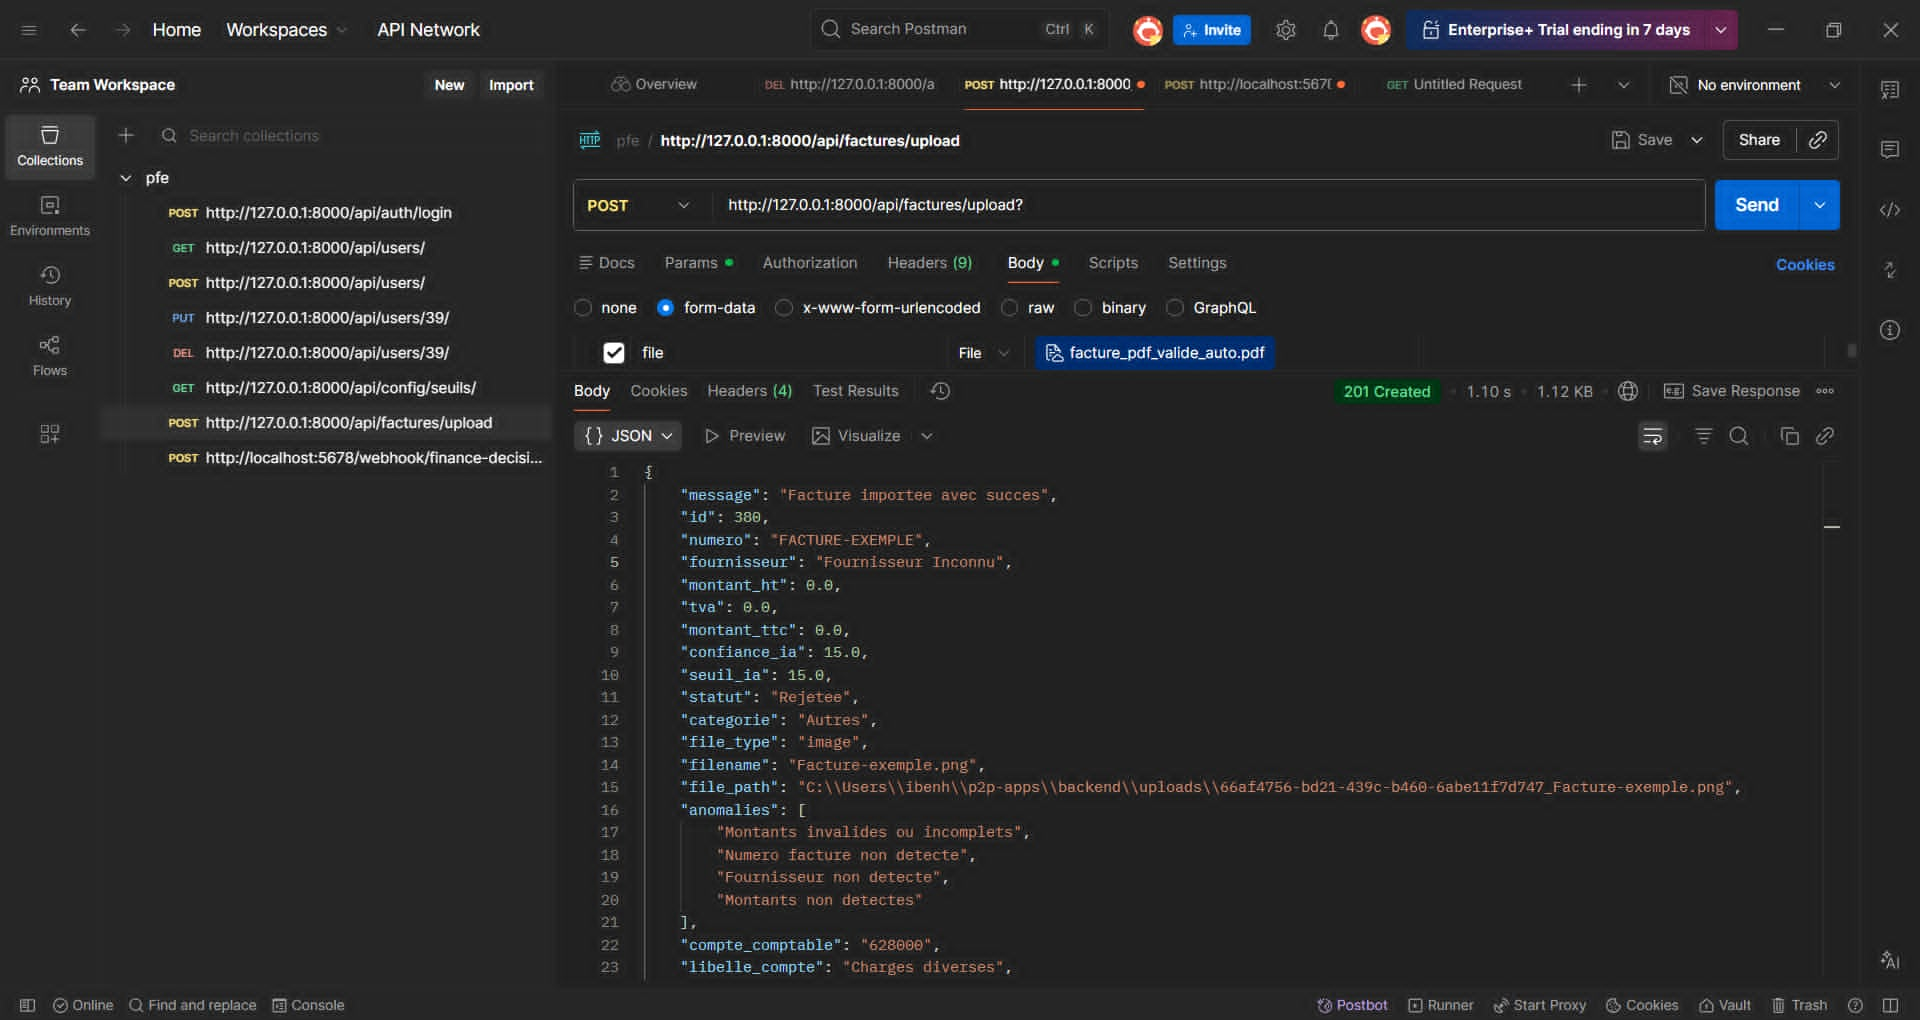
\includegraphics[width=8cm]{figures/postman_import_facture.jpg}
	\\ \hline
	
	Cette requête permet de consulter les données extraites des factures après le traitement OCR et IA. 
	Elle vérifie que les informations détectées sont bien récupérées et affichées correctement.
	&
	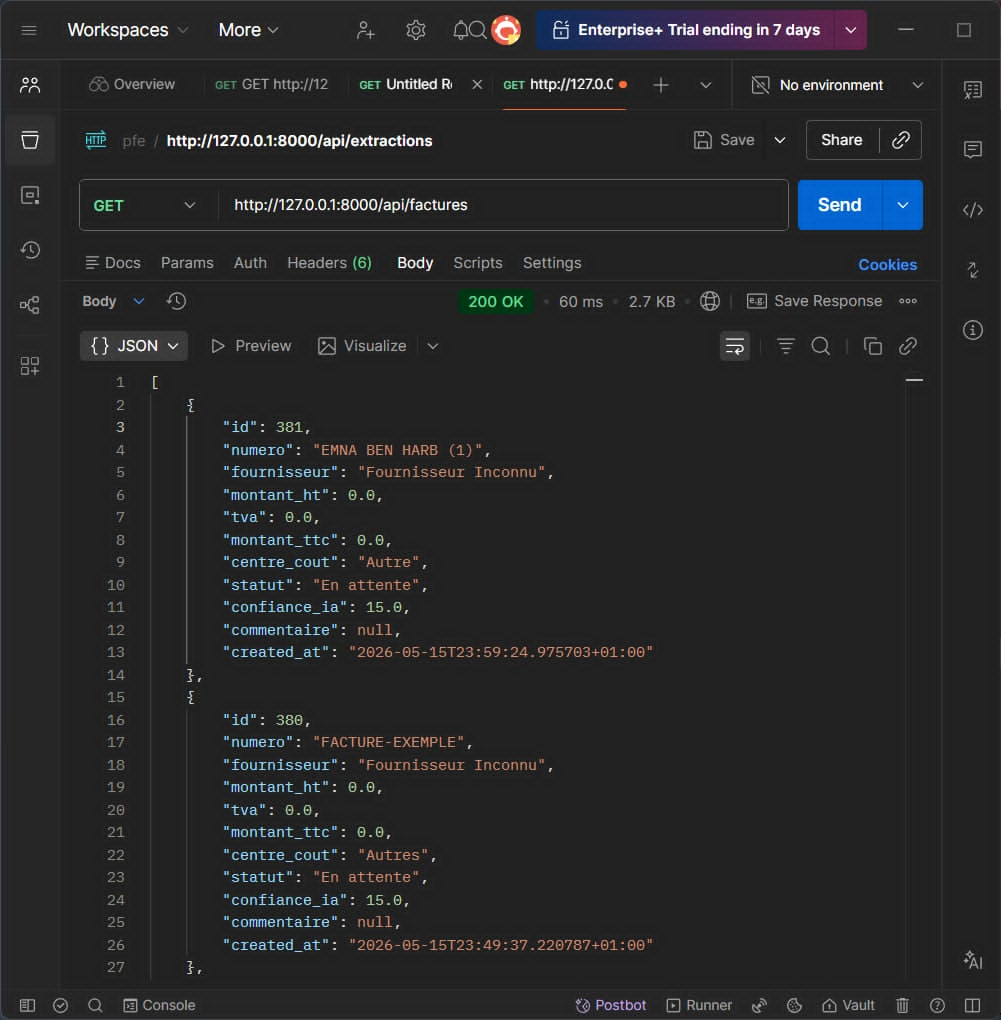
\includegraphics[width=8cm]{figures/postman_resultats.jpg}
	\\ \hline
	
	Cette requête permet de consulter l’historique des actions effectuées dans le système. 
	Elle permet de vérifier la traçabilité des opérations comme l’importation, la modification ou le changement de statut.
	&
	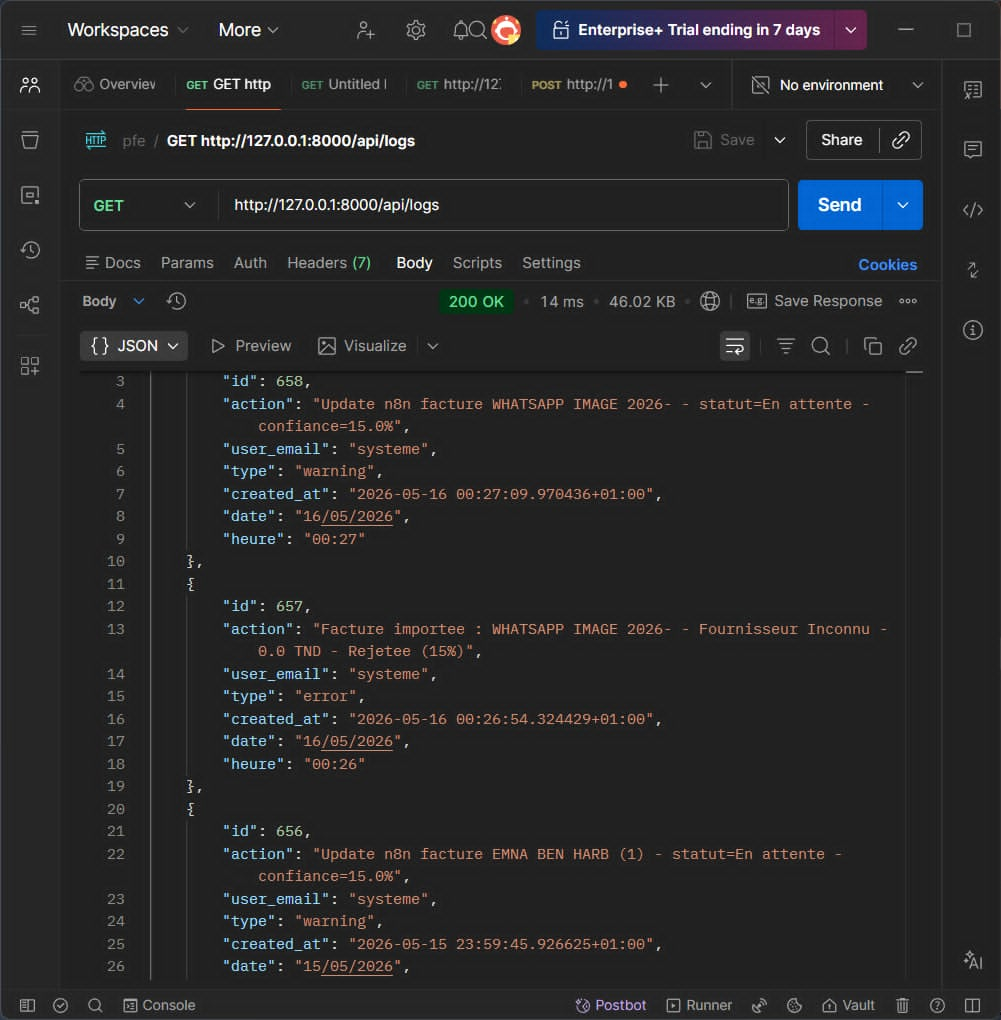
\includegraphics[width=8cm]{figures/postman_logs.jpg}
	\\ \hline
	
	Cette requête permet de récupérer les factures selon leurs statuts. 
	Elle sert à vérifier l’affichage des factures validées, rejetées ou en attente.
	&
	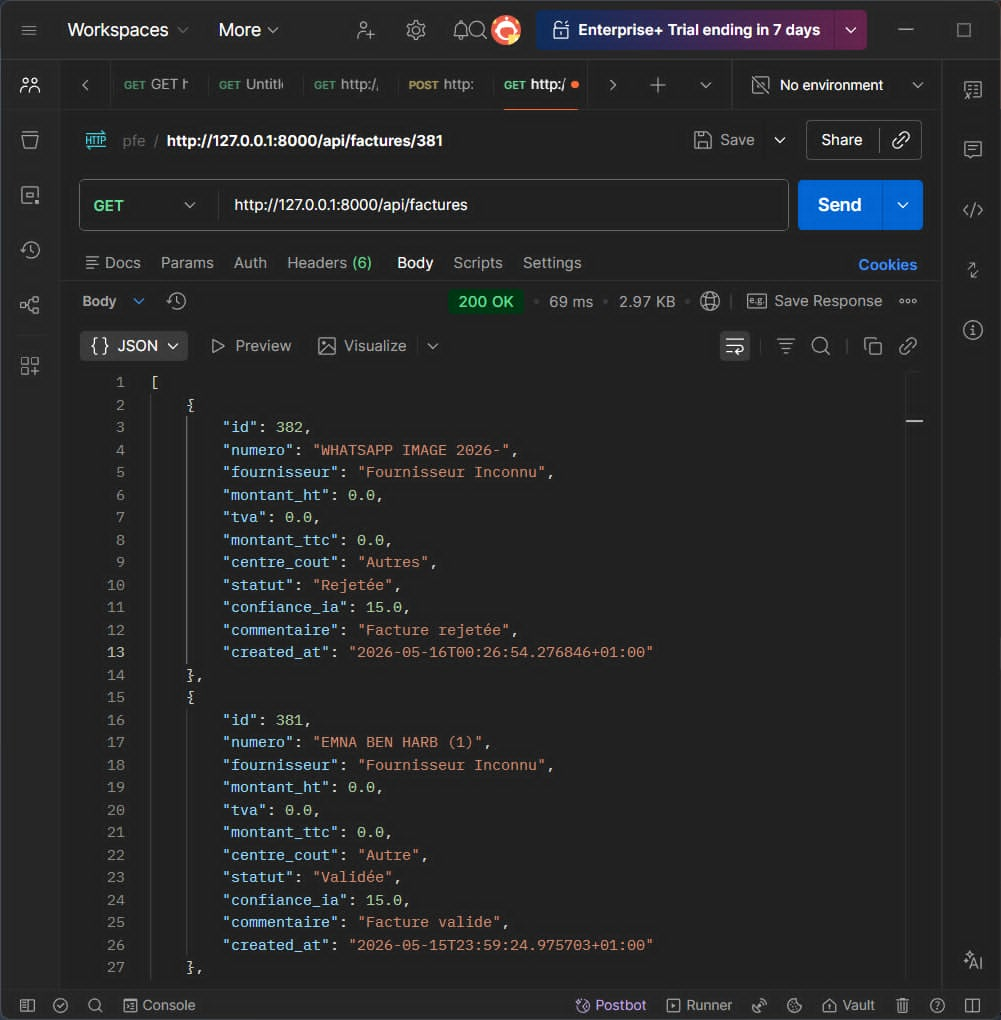
\includegraphics[width=8cm]{figures/postman_factures.jpg}
	\\ \hline
	
	\caption{Tests Postman du Sprint 2}
\end{longtable}
\subsection{Revue de Sprint}

La revue du Sprint 2 a permis de présenter les fonctionnalités développées liées à la gestion des factures, à la consultation des résultats d’extraction ainsi qu’à la visualisation des tableaux de bord et des statistiques. Cette étape a également permis de valider les mécanismes de gestion des statuts
des factures ainsi que la configuration des seuils de confiance de l’intelligence artificielle.
\vspace{0.1cm}
\paragraph{Burndown Chart :}

Le Burndown Chart du Sprint 2 présente l’évolution des tâches relatives au traitement des données, à la consultation des extractions et à la gestion des tableaux de bord. Le graphique illustre la diminution progressive du travail restant jusqu’à la fin du sprint.
Comme présenté dans la figure \ref{fig:brun3}.
\begin{figure}[H]
	\centering
	
\includegraphics[width=0.4\textwidth]{burndown_sprint2.jpg}
	\caption{Diagramme de Burndown Chart du Sprint 2}
	\label{fig:brun2}
\end{figure}
\begin{table}[H]
	\centering
	\renewcommand{\arraystretch}{1.3}
	
	\begin{tabular}{|c|p{5cm}|c|}
		\hline
		\rowcolor{blue!20}
		\textbf{ID User Story} & \textbf{Fonctionnalité} & \textbf{Estimation} \\
		\hline
		
		2.1 & Consultation des données extraites & 3 \\
		\hline
		
		2.2 & Gestion des statuts des factures & 4 \\
		\hline
		
		2.3 & Tableau de bord comptable & 5 \\
		\hline
		
		2.4 & Gestion des anomalies & 3 \\
		\hline
		
		2.5 & Configuration des seuils IA & 4 \\
		\hline
		
		2.6 & Historique des actions & 2 \\
		\hline
		
		\multicolumn{2}{|c|}{\textbf{Vélocité totale estimée}} & \textbf{21} \\
		\hline
		
	\end{tabular}
	
	\caption{Calcul de vélocité estimée du Sprint 2}
\end{table}
\section{Conclusion}

Dans ce chapitre, nous avons présenté les fonctionnalités développées durant le Sprint 2. Nous avons mis en place la gestion des factures, la consultation des résultats d’extraction, les tableaux de bord ainsi que la configuration des seuils de l’intelligence artificielle.